% Inference through Individual Confidential Computing -- Fall 2026 paper
% Compile on Overleaf (pdfLaTeX + BibTeX). Upload this folder as is: main.tex, refs.bib,
% generated/ (from tools/inference_tables.py) and figures/ (from tools/plot_inference.py).
% Every number in the text is a macro from generated/numbers.tex; re-run those two scripts
% after any change to the results instead of editing numbers by hand.
%
% Comments starting "% RAVIV:" mark points that need his ruling before submission.

\documentclass[conference]{IEEEtran}
\IEEEoverridecommandlockouts

\usepackage{amsmath,amssymb,amsthm}
\usepackage{graphicx}
\usepackage{booktabs}
\usepackage{cite}
\usepackage{url}
\usepackage{xcolor}
\usepackage[hidelinks]{hyperref}

\graphicspath{{figures/}}
% generated by tools/inference_tables.py -- do not edit
\newcommand{\NRuns}{727}
\newcommand{\NScores}{90{,}311}
\newcommand{\NExactRuns}{727}
\newcommand{\NViolations}{0}
\newcommand{\NSRuns}{396}
\newcommand{\NFRuns}{288}
\newcommand{\NRRuns}{36}
\newcommand{\SMaxErrOverBound}{1.00}
\newcommand{\SMaxErrClean}{4.1\times10^{-2}}
\newcommand{\SMaxErrOverBoundClean}{0.73}
\newcommand{\SMeanErrOverBoundClean}{0.16}
\newcommand{\SNClippedRuns}{174}
\newcommand{\SMaxErrClipped}{261}
\newcommand{\SMaxGapLin}{0.409}
\newcommand{\SMaxGapLinClean}{9.9\times10^{-4}}
\newcommand{\SNCleanLin}{72}
\newcommand{\SMaxGapLog}{2.0\times10^{-2}}
\newcommand{\SMaxGapLogClean}{1.0\times10^{-2}}
\newcommand{\SNCleanLog}{74}
\newcommand{\SFlipsLog}{34}
\newcommand{\SDecisionsLog}{13{,}200}
\newcommand{\SMaxGapSoft}{3.0\times10^{-2}}
\newcommand{\SMaxGapSoftClean}{1.0\times10^{-2}}
\newcommand{\SNCleanSoft}{76}
\newcommand{\SFlipsSoft}{47}
\newcommand{\SDecisionsSoft}{13{,}200}
\newcommand{\SFlipsOutsideBound}{0}
\newcommand{\SMaxErrUnclippedRows}{4.1\times10^{-2}}
\newcommand{\SMoverNMin}{0.54}
\newcommand{\SMoverNMax}{0.69}
\newcommand{\SHMin}{0.31}
\newcommand{\SHMax}{0.49}
\newcommand{\SSpikedH}{0.03}
\newcommand{\SSpikedMoverN}{0.98}
\newcommand{\SDiscH}{0.07}
\newcommand{\SDiscMoverN}{0.94}
\newcommand{\SLogQMin}{20.0}
\newcommand{\SLogQMax}{25.3}
\newcommand{\EpsCMin}{1.3\times10^{-3}}
\newcommand{\EpsCMax}{3.9\times10^{-3}}
\newcommand{\EpsCAltMax}{3.9\times10^{-3}}
\newcommand{\EpsCBitsMax}{4.5\times10^{-2}}
\newcommand{\CN}{442}
\newcommand{\Cn}{4{,}420}
\newcommand{\CLam}{2{,}483}
\newcommand{\CDTwoLam}{6{,}564{,}876}
\newcommand{\CRatio}{2{,}644}
\newcommand{\CTotal}{151}
\newcommand{\CPerScore}{130}
\newcommand{\RDiabFloat}{0.5156}
\newcommand{\RDiabScheme}{0.5173}
\newcommand{\RDiabM}{1{,}656}
\newcommand{\RDiabLam}{1{,}657}
\newcommand{\RDiabn}{2{,}210}
\newcommand{\RDiabH}{0.254}
\newcommand{\RDiabLogQ}{22.3}
\newcommand{\RDiabClipped}{2}
\newcommand{\RDiabFlips}{0}
\newcommand{\RDiabErrMax}{0.1816}
\newcommand{\RDiabWall}{29}
\newcommand{\RDiabMoverN}{0.75}
\newcommand{\RDiabN}{221}
\newcommand{\RDiabP}{10}
\newcommand{\RDiabQueries}{221}
\newcommand{\RDiabDownload}{366{,}197}
\newcommand{\RDiabDecryptDownload}{3{,}661{,}970}
\newcommand{\RWineFloat}{0.9438}
\newcommand{\RWineScheme}{0.9551}
\newcommand{\RWineM}{825}
\newcommand{\RWineLam}{826}
\newcommand{\RWinen}{1{,}157}
\newcommand{\RWineH}{0.292}
\newcommand{\RWineLogQ}{22.7}
\newcommand{\RWineClipped}{2}
\newcommand{\RWineFlips}{1}
\newcommand{\RWineErrMax}{1.007}
\newcommand{\RWineWall}{13}
\newcommand{\RWineMoverN}{0.71}
\newcommand{\RWineN}{89}
\newcommand{\RWineP}{13}
\newcommand{\RWineQueries}{267}
\newcommand{\RWineDownload}{220{,}542}
\newcommand{\RWineDecryptDownload}{955{,}682}


\newtheorem{observation}{Observation}
\newtheorem{proposition}{Proposition}
\theoremstyle{remark}
\newtheorem{remark}{Remark}

\newcommand{\F}{\mathbb{F}}
\newcommand{\xt}{\tilde{x}}
\newcommand{\xh}{\hat{x}}
\newcommand{\wh}{\hat{w}}
\newcommand{\bh}{\hat{b}}
\newcommand{\clip}{\operatorname{clip}}
\newcommand{\todo}[1]{\textcolor{red}{[#1]}}

\begin{document}

\title{Private Inference on Stored Non-Uniform Data\\ with Individual Confidential Computing}

\author{\IEEEauthorblockN{Daniel Palmer}
\IEEEauthorblockA{Department of Computer Science and Engineering\\
Washington University in St.\ Louis}}

\maketitle

% ─────────────────────────────────────────────────────────────────────────────
\begin{abstract}
Individual Confidential Computing (ICC) lets a client store non-uniformly distributed data
with an untrusted provider and later have the provider evaluate low-degree polynomials of
it, while no $r$ of the stored values leak more than a negligible amount of information to
the provider as a whole. We study ICC in an inference setting: the data are stored once, a
linear, logistic or softmax model trained elsewhere is applied to every stored row, and the
requests are independent of the data. We show that this setting inherits the scheme's
guarantee unchanged, that the model's scores are degree-one queries whose fixed-point
encoding yields an explicit field size and an explicit error bound, and that degree one
keeps the number of workers linear in the data size. In \NRuns{} end-to-end runs covering
\NScores{} scores over eleven synthetic sources, a grid of fixed-point formats, and two
real datasets, every score decoded exactly to its integer value and the measured error
never exceeded the analytic bound. Without clipping, task metrics matched the floating-point
model to within $10^{-3}$ in $R^2$ and one decision per hundred rows; the larger
deviations all came from clipping heavy-tailed features, which the bound predicts and the
client controls by the choice of clip. On the
diabetes dataset the scheme reaches $R^2=\RDiabScheme$ against $\RDiabFloat$ in floating
point, and on wine an accuracy of $\RWineScheme$ against $\RWineFloat$, using
$\RDiabLam$ and $\RWineLam$ workers respectively. At the same data size, a degree-two
gradient query, as training would need, requires $\CRatio\times$ more workers.
\end{abstract}

% ─────────────────────────────────────────────────────────────────────────────
\section{Introduction}

A client who stores data with a cloud provider would like the provider to compute on it
without learning it. Homomorphic encryption achieves this computationally
\cite{cryptonets2016}; coded computing achieves information-theoretic guarantees by
spreading encoded data over many workers \cite{yu2019lcc}. The perfect subset privacy
line of work \cite{raviv2022,deng2024} asks for less than full secrecy and gets more
efficiency in return: no $r$-subset of the data may be learned by the provider as a whole,
admin and workers together. Individual Confidential Computing (ICC) \cite{icc2025} removes
the remaining requirement that the data be uniform, replacing zero leakage by a negligible
leakage $\varepsilon_c$ through distribution smoothing \cite{pathegama2024}.

Earlier work on this implementation found that real-valued data can be carried into the
finite field by a fixed-point encoding with a hard no-wraparound guarantee. This paper asks
where that makes ICC useful today. Iterative training is not yet covered: in gradient
descent each query depends on the previous decoded gradient, so the query coefficients form
a data-dependent channel outside the theorem. \emph{Inference} is covered. A model trained
elsewhere is public, its scores on stored rows are fixed in advance, and each score is a
degree-one polynomial of the stored data.

\textbf{Contributions.}
\begin{itemize}
\item We state the conditions under which inference adds no leakage beyond the ICC storage
      guarantee (Section~\ref{sec:setting}): a model not fitted on the stored rows,
      preprocessing statistics taken from training rows, and non-adaptive requests.
\item We give the fixed-point encoding of linear, logistic and softmax scores, the field
      size that rules out wraparound, and a deterministic bound on the score error
      (Section~\ref{sec:encoding}).
\item We measure the full pipeline end to end on synthetic sources with exact entropies, on
      a grid of formats, and on two real datasets (Sections~\ref{sec:setup}
      and~\ref{sec:results}), and compare its cost with the degree-two query training would
      need.
\end{itemize}

% ─────────────────────────────────────────────────────────────────────────────
\section{The ICC scheme}\label{sec:icc}

The client holds $x\in\F_q^n$ drawn from an unknown, non-uniform distribution. To store it,
the client draws a key $k\sim\mathrm{Unif}(\F_q^m)$ and a random matrix
$G\in\F_q^{m\times n}$, uploads $\xt = x + kG$ together with $G$, and keeps only $k$
\cite{icc2025}. The provider's admin gives one worker the share $\xt - tG$ for each $t$ in
an information set $I_{d,m}$ of the Reed--Muller code $\mathrm{RM}_q(d,m)$; there are
$\lambda=|I_{d,m}|=\binom{m+d}{d}$ workers when $d<q$ \cite{deng2024}. To evaluate a
polynomial $f$ of total degree at most $d$, each worker returns $f(\xt-tG)$. The function
$g(t)\triangleq f(\xt-tG)$ is a polynomial of degree at most $d$ in $t$, so the client
interpolates it from the $\lambda$ returns and outputs $g(k)=f(x)$.

\textbf{Key length.} Let $H_p$ denote R\'enyi entropy of order $p\ge2$ in base $q$.
Theorem~1 of \cite{icc2025} guarantees $I(X_R;\xt)\le\varepsilon_c$ for every
$R\subseteq[n]$, $|R|=r$, with probability at least $1-1/a$ over $G$, provided
\begin{equation}\label{eq:m}
m \ge n + p + \log_q(1/\varepsilon) - H_p(X) + \max_{R} H_p(X_R),
\end{equation}
where $\varepsilon$ is the smoothing budget and
$\varepsilon_c=\tfrac{p}{p-1}\log_q\!\big(1+a\,2^{(2p-1)/p}(1+q^{-\max_R H_p(X_R)})\varepsilon^{1/p}\big)$.
% RAVIV: known issue 1 -- the derivation at eqs. (9)-(10) of [icc2025] carries
% q^{-max_R H_p(X_R)/p}. We report both; they agree to the digits shown (EpsCAltMax).
The more entropy the data carry, the shorter the key: writing $h=H_p(X)/n$, the key length
is roughly $m\approx n(1-h)$.

% ─────────────────────────────────────────────────────────────────────────────
\section{Inference setting}\label{sec:setting}

The client stores $N$ rows of $P$ features, $n=NP$ values, once. A model with $K$ outputs,
weights $W\in\mathbb{R}^{K\times P}$ and intercepts $b\in\mathbb{R}^K$, has been trained
elsewhere ($K=1$ for linear and binary logistic regression, $K$ classes for softmax). For
every stored row $i$ and output $c$ the client wants the score
$z_{ic}=w_c^\top x_i+b_c$; the link (identity, sigmoid or softmax) is applied by the client
after decoding, so it never needs to be a polynomial. The model is public: its weights are
the coefficients of the query polynomial the provider evaluates.

\begin{observation}\label{obs:inference}
Suppose the query polynomials $f_1,\dots,f_Q$ are independent of $(X,k)$. Then the
provider's view after answering all of them satisfies
$I(X_R;\text{view})=I(X_R;\xt,G)\le\varepsilon_c$.
\end{observation}
\begin{proof}
Every worker output $f_j(\xt-tG)$ is a deterministic function of $(\xt,G,f_j)$, so the
view is a function of $(\xt,G,f_1,\dots,f_Q)$. Since $(f_1,\dots,f_Q)$ is independent of
$(X,\xt,G)$, the chain rule gives $I(X_R;\xt,G,f_{1:Q})=I(X_R;\xt,G)$.
\end{proof}
% RAVIV: this is the data-processing argument we discussed; no new lemma intended.

Three rules make the hypothesis hold in practice:
\begin{enumerate}
\item the model is not fitted on the stored rows (we use a train/store split, or fresh
      synthetic draws);
\item preprocessing statistics, such as standardisation means and deviations, are
      computed on the training rows only;
\item the requests are not adaptive: which rows are scored, and by which model, is fixed
      before any result is decoded.
\end{enumerate}
Live gradient descent violates the third rule, which is why it is left to future work.

% ─────────────────────────────────────────────────────────────────────────────
\section{Fixed-point encoding of scores}\label{sec:encoding}

\textbf{Codes.} A feature is clipped to $[-A_X,A_X]$ and stored as the integer
$\xh=\mathrm{round}(2^{f_X}\clip(x))$, mapped into $\F_q$ by its balanced representative.
Weights and intercepts are coded with $f_w$ fractional bits,
$\wh=\mathrm{round}(2^{f_w}w)$, $\bh=\mathrm{round}(2^{f_w}b)$, with public clips $A_w,A_b$
covering the model. The query for row $i$ and output $c$ is
\begin{equation}\label{eq:query}
\hat z_{ic}=\sum_{j=1}^{P}\wh_{cj}\,\xh_{ij}+2^{f_X}\,\bh_c ,
\end{equation}
a degree-one polynomial in the stored values with public integer coefficients, equal to
$2^{f_X+f_w}$ times the dequantised score. One upload serves every row and output.

\textbf{Field size.} Decoding returns $\hat z_{ic}\bmod q$; it equals the integer
$\hat z_{ic}$ whenever $|\hat z_{ic}|\le (q-1)/2$. With
$\hat X_{\max}=2^{f_X}A_X$, $\hat W_{\max}=2^{f_w}A_w$, $\hat B_{\max}=2^{f_w}A_b$,
\begin{equation}\label{eq:B}
|\hat z_{ic}|\le B\triangleq P\,\hat X_{\max}\hat W_{\max}+2^{f_X}\hat B_{\max},
\end{equation}
so any prime $q>2B$ guarantees an exact integer. The provider checks this bound before
dispatching a query and refuses otherwise. For $P=10$, $f_X=f_w=8$, $A_X=4$, $A_w=2$,
$A_b=1$, $B\approx5.3\times10^6$ and $q\approx2^{23.3}$.

\begin{proposition}[score error]\label{prop:err}
Let $z=w^\top x+b$ be the floating-point score and $z_{\mathrm{s}}=\hat z/2^{f_X+f_w}$ the
decoded one. Then
\begin{multline*}
|z_{\mathrm{s}}-z|\le\sum_j|w_j|\big(|x_j-\clip(x_j)|+2^{-f_X-1}\big)\\
+2^{-f_w-1}\textstyle\sum_j|\clip(x_j)|+P\,2^{-f_X-f_w-2}+2^{-f_w-1}.
\end{multline*}
\end{proposition}
\begin{proof}
Write $\xh_j/2^{f_X}=\clip(x_j)+\delta_j$ and $\wh_j/2^{f_w}=w_j+\gamma_j$ with
$|\delta_j|\le2^{-f_X-1}$, $|\gamma_j|\le2^{-f_w-1}$, and likewise $\gamma_b$ for the
intercept. Expanding, $z_{\mathrm{s}}-z=\sum_j[w_j(\clip(x_j)-x_j)+w_j\delta_j+\gamma_j
\clip(x_j)+\gamma_j\delta_j]+\gamma_b$, and the triangle inequality gives the claim. Since
decoding is exact, no other error source exists.
\end{proof}

The first term is the clipping error; it vanishes unless a feature lies outside
$\pm A_X$. All other terms halve with every extra fractional bit. For classification, a
decision (sign or argmax) can change only for rows whose floating-point margin is within
the bound of a tie.

\textbf{Entropy and key length at degree one.} The field is sized by the product of data
and weight magnitudes, so $\log_2 q$ grows with $f_w$, while the entropy of the stored codes
depends on the data alone. For a standard Gaussian at $f_X=8$, $A_X=4$, the order-2 entropy
is about $9.8$ bits per code against $\log_2 q\approx22$, so $h\approx0.45$ and
$m\approx0.55\,n$. The gain in exactness from a larger $f_w$ is paid for in key length.

% ─────────────────────────────────────────────────────────────────────────────
\section{Experimental setup}\label{sec:setup}

Every run uploads the stored rows through the scheme, sends one query~\eqref{eq:query} per
row and output, decodes all scores with a single interpolation, and compares every decoded
integer with the plaintext integer oracle. Privacy settings are $r=5$, $p=2$,
$\varepsilon=10^{-6}$, $a=5$. The implementation uses \texttt{galois} \cite{galois} and
scikit-learn \cite{sklearn}; all runs are seeded and their raw output is saved.

\textbf{Synthetic sources (S).} Nine i.i.d.\ feature families (Gaussian, uniform, bimodal,
three-point discrete, Laplace, Student-$t_3$, spiked, exponential, lognormal) and
equicorrelated Gaussians with $\rho\in\{0.5,0.9\}$; tasks linear, logistic and three-class
softmax; $P\in\{2,5,10,20\}$; $N=100$ stored rows; $f_X=f_w=8$, $A_X=4\sigma$; three seeds,
\NSRuns{} runs. Models are fitted on 2{,}000 independent training rows (least squares, or
$L_2$-regularised logistic regression). For i.i.d.\ sources $H_p(X)$ and
$\max_R H_p(X_R)$ are computed exactly from the code distribution; for correlated sources
we use a min-entropy lower bound on $H_p(X)$ and the model-free upper bound
$\max_R H_p(X_R)\le r\log_q(\text{levels})$.

\textbf{Formats (F).} $f_X,f_w\in\{2,4,\dots,12\}$ on Gaussian and lognormal features,
linear and logistic, $P=10$, $N=50$, two seeds (\NFRuns{} runs).

\textbf{Cost (C).} Gaussian linear model, $P=10$, $N$ from 10 to 442 (the size of the
diabetes data), with the degree-two training plan for the same data computed alongside.

\textbf{Real data (R).} Diabetes \cite{efron2004lars} (442 rows, 10 features, regression)
and wine \cite{uciwine} (178 rows, 13 features, 3 classes), each shuffled with a public seed
and split in half: the model is fitted and standardisation statistics are computed on the
first half, and the second half is stored and scored. Formats
$f_X,f_w\in\{4,6,8\}$ and $A_X\in\{4\sigma,8\sigma\}$ (\NRRuns{} runs).

\textbf{Real-data entropy (provisional).} Real features are correlated, and R\'enyi entropy
of order $p\ge2$ is not subadditive, so a sum of per-feature entropies bounds $H_p(X)$ in
neither direction. We lower-bound the entropy of a stored row by its min-entropy,
$\sum_j \min(f_X,b_j)-\log_2\rho_{\max}$, where $\rho_{\max}$ is the peak of a Gaussian
density fitted to the training half, $b_j=\log_2(\sigma_j/s_j)$ caps the bits of a
feature recorded on a grid of step $s_j$, and discrete features are credited zero bits.
% RAVIV: the Gaussian rho_max is a model, not a guarantee. Needs a ruling (CLAUDE.md
% known issues 2-3; docs/INFERENCE.md section 6).
This bound is provisional: the Gaussian peak is a modelling assumption.

% ─────────────────────────────────────────────────────────────────────────────
\section{Results}\label{sec:results}

\subsection{Exactness and the error bound}

All \NExactRuns{} of \NRuns{} runs decoded every score exactly to its integer value, over
\NScores{} scores in total. Fig.~\ref{fig:bound} compares the measured error with
Proposition~\ref{prop:err}: there were \NViolations{} violations. Without clipping, the
largest score error was $\SMaxErrClean$ and at most $\SMaxErrOverBoundClean$ of the bound
(the mean error is $\SMeanErrOverBoundClean$ of the mean bound). In the \SNClippedRuns{}
synthetic runs where some feature fell outside $\pm4\sigma$, the clipping term dominates
and the bound is nearly tight. The largest error, $\SMaxErrClipped$, came from two
Student-$t_3$ values far outside the clip; on the rows of every run with no clipped feature
the error stayed below $\SMaxErrUnclippedRows$.

\begin{figure}[t]
\centering
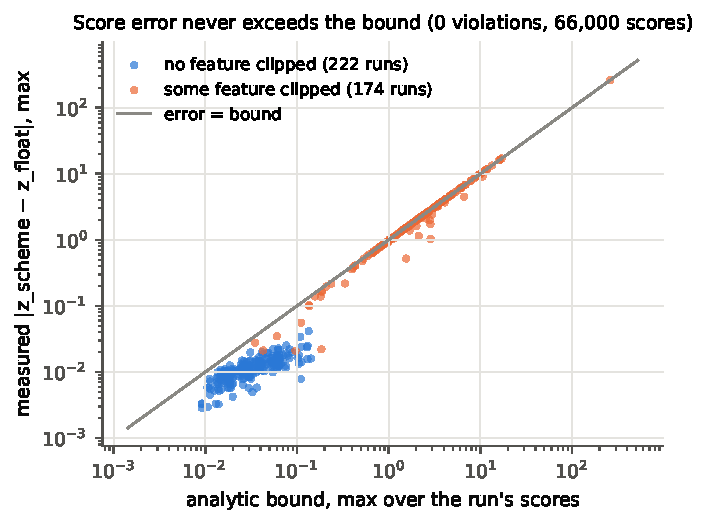
\includegraphics[width=\columnwidth]{fig2_error_vs_bound}
\caption{Measured maximum score error against the bound of
Proposition~\ref{prop:err}, one point per synthetic run.}
\label{fig:bound}
\end{figure}

\subsection{Task metrics across sources}

Fig.~\ref{fig:metrics} plots each run's metric through the scheme against the
floating-point model. In runs with no clipped feature the largest gap was
$\SMaxGapLinClean$ in $R^2$ (\SNCleanLin{} linear runs) and $\SMaxGapLogClean$ and
$\SMaxGapSoftClean$ in accuracy for logistic and softmax, that is, at most one of 100
decisions. With clipping the gaps reach $\SMaxGapLin$ in $R^2$ (Student-$t_3$),
$\SMaxGapLog$ and $\SMaxGapSoft$ in accuracy: the heavy-tailed and skewed sources
(Laplace, Student-$t_3$, exponential, lognormal, spiked) put values beyond $4\sigma$, and a
$4\sigma$ clip is the wrong choice for them. Decisions flipped on
\SFlipsLog{} of \SDecisionsLog{} logistic rows and \SFlipsSoft{} of \SDecisionsSoft{}
softmax rows, and every flip occurred on a row the bound flagged as near a tie
(\SFlipsOutsideBound{} outside it). Table~\ref{tab:sources} summarises each source.

\begin{figure*}[t]
\centering
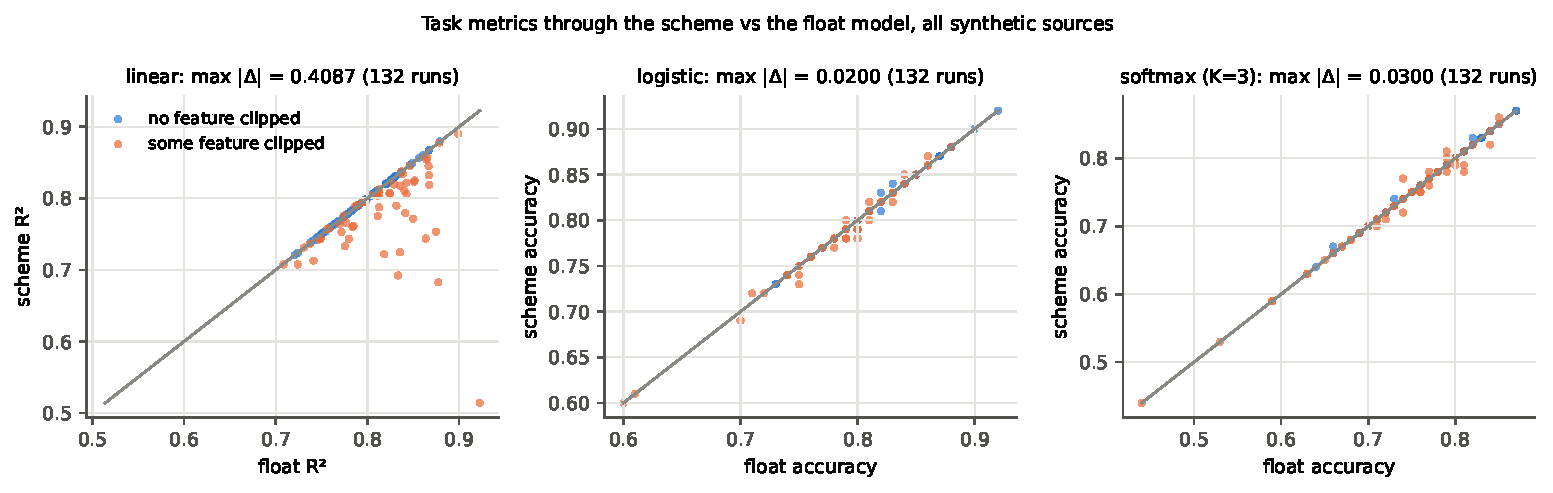
\includegraphics[width=\textwidth]{fig5_metrics}
\caption{Task metric through the scheme against the floating-point model, all synthetic
runs. Orange: runs in which some feature was clipped.}
\label{fig:metrics}
\end{figure*}

\begin{table}[t]
\centering
\caption{Per-source summary of experiment S (all tasks and $P$ pooled).}
\label{tab:sources}
\resizebox{\columnwidth}{!}{\begin{tabular}{lrrrrrr}
\toprule
source & $h$ & $m/n$ & clipped & max err & $\max|\Delta R^2|$ & flips \\
\midrule
gauss & 0.44 & 0.57 & 2 & 0.035 & $9.9\times10^{-4}$ & 2/2400 \\
gauss ($\rho=0.5$) & 0.40 & 0.62 & 3 & 0.219 & $1.0\times10^{-3}$ & 2/2400 \\
gauss ($\rho=0.9$) & 0.35 & 0.66 & 2 & 0.041 & $7.1\times10^{-4}$ & 1/2400 \\
uniform & 0.44 & 0.58 & 0 & 0.023 & $3.7\times10^{-4}$ & 1/2400 \\
bimodal & 0.43 & 0.58 & 0 & 0.022 & $5.1\times10^{-4}$ & 2/2400 \\
discrete3 & 0.07 & 0.94 & 0 & 0.022 & $7.5\times10^{-4}$ & 2/2400 \\
laplace & 0.42 & 0.59 & 128 & 4.786 & $1.9\times10^{-2}$ & 9/2400 \\
student3 & 0.41 & 0.60 & 202 & 260.702 & $0.409$ & 5/2400 \\
spiked & 0.03 & 0.98 & 469 & 4.681 & $3.6\times10^{-2}$ & 18/2400 \\
exponential & 0.39 & 0.62 & 639 & 6.295 & $7.9\times10^{-2}$ & 15/2400 \\
lognormal & 0.38 & 0.63 & 722 & 15.972 & $0.195$ & 24/2400 \\
\bottomrule
\end{tabular}
}
\end{table}

\subsection{Choice of format}

Fig.~\ref{fig:format} shows the format grid. The error falls by half per extra bit until
the other term dominates: extra weight bits do not help while $f_X$ is small, and vice
versa. For lognormal features the clipping error at $A_X=4\sigma$ dominates every format.
Fig.~\ref{fig:formatcost} shows the price: $\log_2 q$ grows by one per extra bit of either
kind. The key length moves in opposite directions: $m/n$ grows with $f_w$, because weight
bits enlarge the field without adding entropy, and falls with $f_X$, because data bits add
entropy as fast as they enlarge the field. Balanced formats are therefore efficient. On
Gaussian features $f_X=f_w=6$ already keeps the $R^2$ gap below $10^{-3}$ at
$\log_2 q\approx18$, and $f_X=f_w=8$ ($\log_2 q\approx22$) brings the maximum score
error to about $10^{-2}$; we use the latter as the default.

\begin{figure*}[t]
\centering
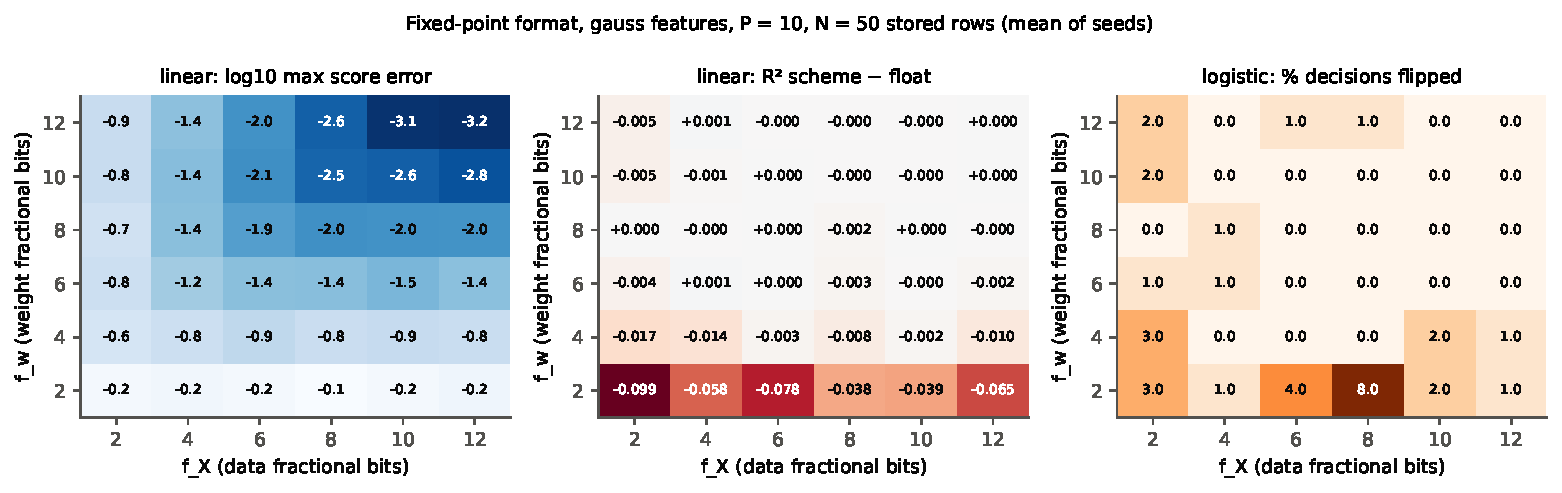
\includegraphics[width=\textwidth]{fig3_format_gauss}
\caption{Format grid on Gaussian features ($P=10$, $N=50$, mean of two seeds).}
\label{fig:format}
\end{figure*}

\begin{figure}[t]
\centering
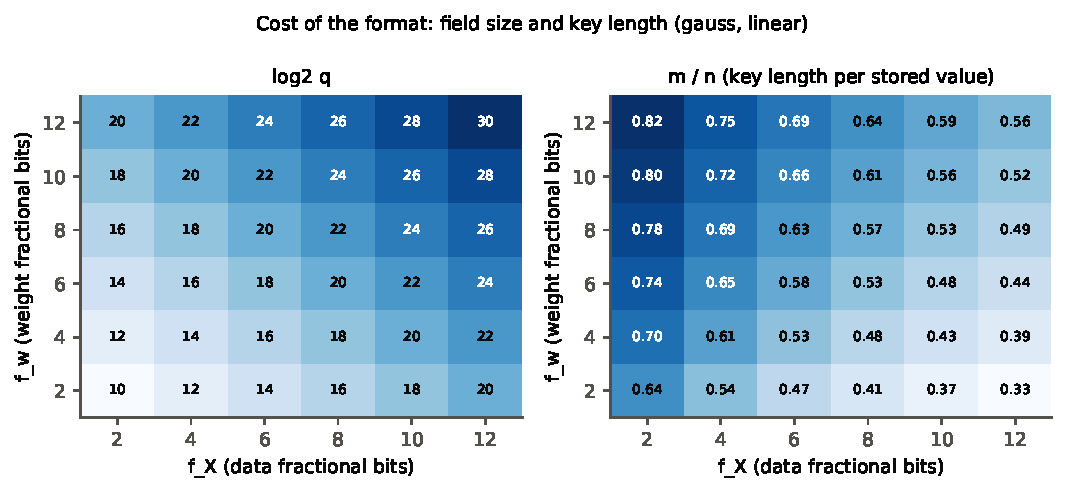
\includegraphics[width=\columnwidth]{fig3c_format_cost}
\caption{Field size and key length over the format grid.}
\label{fig:formatcost}
\end{figure}

\subsection{Key length}

Across the continuous synthetic sources, $h$ ranged from $\SHMin$ to $\SHMax$ and $m/n$
from $\SMoverNMin$ to $\SMoverNMax$ (Fig.~\ref{fig:keylen}); correlation lowers $h$ and
lengthens the key, partly because correlated sources are sized by the looser bounds
route. Two low-entropy sources need a key almost as long as the data: the
three-point discrete source ($h=\SDiscH$, $m/n=\SDiscMoverN$) and the spiked source, with
most of its mass on one value ($h=\SSpikedH$, $m/n=\SSpikedMoverN$). Little entropy means
little to smooth with, and the points follow $m/n\approx1-h$ closely. The
leakage bound $\varepsilon_c$ ranged from $\EpsCMin$ to $\EpsCMax$ in $\log_q$ units.

\begin{figure*}[t]
\centering
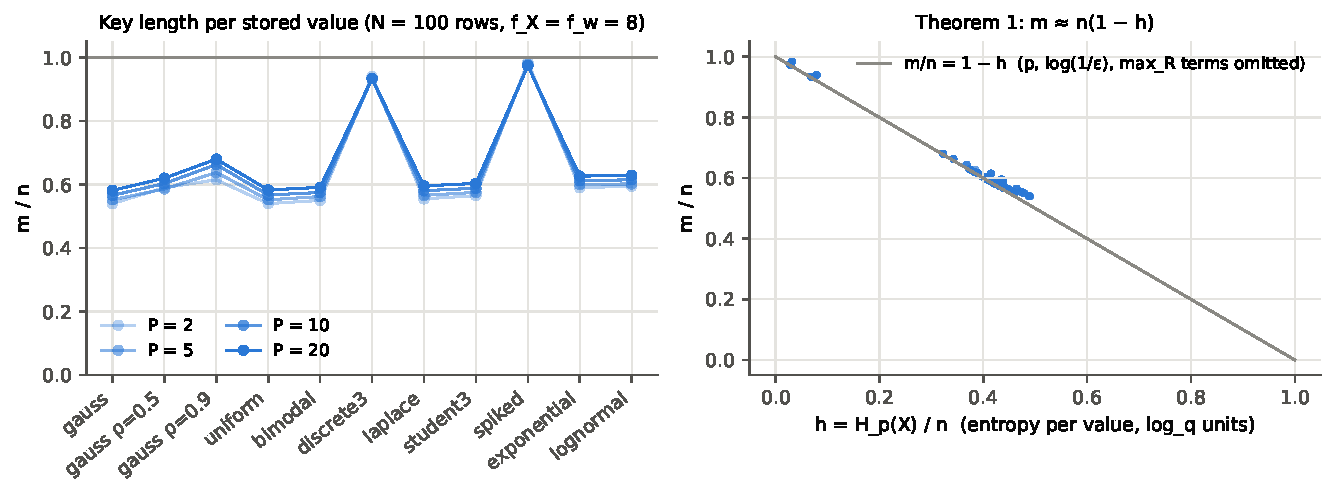
\includegraphics[width=\textwidth]{fig4_key_length}
\caption{Key length per stored value across sources (left) and against the entropy per
value (right).}
\label{fig:keylen}
\end{figure*}

\subsection{Cost: inference versus training queries}

At degree one, $\lambda=m+1$ grows linearly with the data. Table~\ref{tab:cost} and
Fig.~\ref{fig:cost} show the measured cost. At $N=\CN$ rows ($n=\Cn$) the scheme used
$\CLam$ workers, while a degree-two least-squares gradient query on the same data would need
$\lambda=\binom{m+2}{2}=\CDTwoLam$, about $\CRatio\times$ more. The complete run at that size,
from upload to all decoded scores, took about \CTotal{}~s, split roughly evenly between
building the shares (37~s), building the interpolation matrix once (56~s) and evaluating
the $\CN$ queries on every worker (54~s); decoding all scores took 3~s. The matrix is
reused by every later request on the same upload.

A practical limit comes from the arithmetic library. Its matrix product falls back to
Python integers when the inner dimension times $q^2$ exceeds $2^{63}$: at $n=4{,}420$
storing took 28.8~s at $\log_2 q=24$ but 872.9~s at $\log_2 q=27$. The default formats keep
$\log_2 q$ near 22--24.

\begin{table}[t]
\centering
\caption{Cost against stored size ($P=10$, $f_X=f_w=8$).}
\label{tab:cost}
\resizebox{\columnwidth}{!}{\begin{tabular}{rrrrrrrrr}
\toprule
$N$ & $n$ & $\log_2 q$ & $m$ & $\lambda$ & store & eval & decode & $\lambda$ at $d{=}2$ \\
& & & & & (s) & (s) & (s) & (plan) \\
\midrule
10 & 100 & 22.3 & 62 & 63 & 0.00 & 0.03 & 0.01 & 3{,}486 \\
25 & 250 & 22.3 & 146 & 147 & 0.00 & 0.18 & 0.02 & 20{,}503 \\
50 & 500 & 22.3 & 286 & 287 & 0.01 & 0.71 & 0.04 & 81{,}003 \\
100 & 1{,}000 & 22.3 & 566 & 567 & 0.14 & 2.76 & 0.12 & 326{,}028 \\
200 & 2{,}000 & 22.3 & 1{,}126 & 1{,}127 & 2.04 & 11.24 & 0.42 & 1{,}321{,}125 \\
300 & 3{,}000 & 22.3 & 1{,}686 & 1{,}687 & 7.00 & 25.10 & 0.98 & 3{,}000{,}025 \\
442 & 4{,}420 & 22.3 & 2{,}482 & 2{,}483 & 37.06 & 54.10 & 3.21 & 6{,}564{,}876 \\
\bottomrule
\end{tabular}
}
\end{table}

\begin{figure*}[t]
\centering
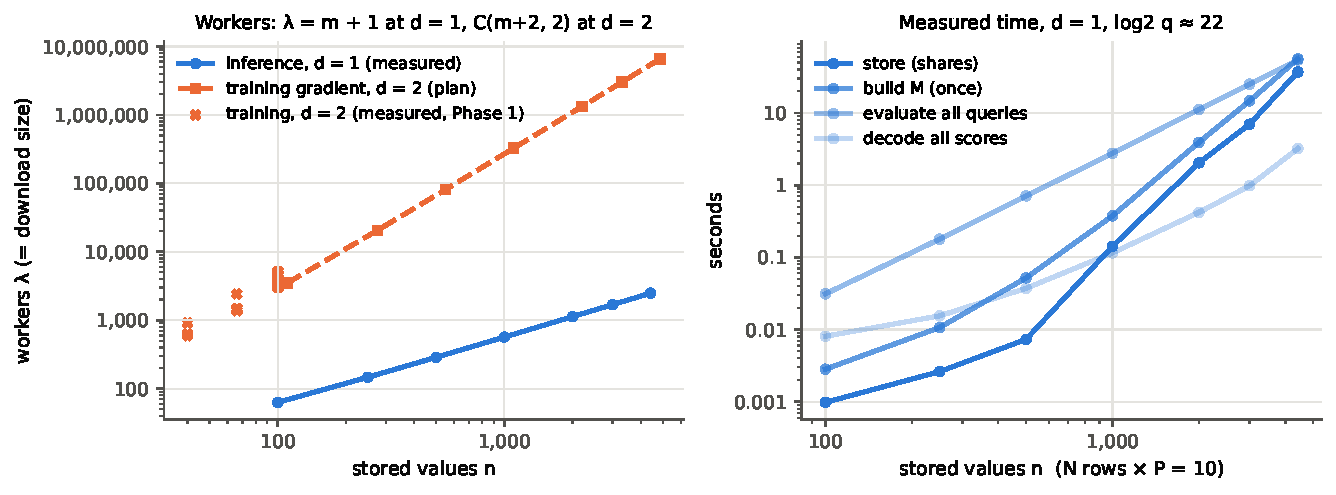
\includegraphics[width=\textwidth]{fig6_cost}
\caption{Workers (left) and measured time per phase (right) against stored size.}
\label{fig:cost}
\end{figure*}

\subsection{Real data}

Fig.~\ref{fig:real} shows every stored row of both datasets at $f_X=f_w=8$,
$A_X=4\sigma$. On diabetes ($n=\RDiabn$, $\log_2 q=\RDiabLogQ$, $h=\RDiabH$,
$m=\RDiabM$), $R^2$ through the scheme was $\RDiabScheme$ against $\RDiabFloat$ in
floating point. On wine ($n=\RWinen$, $h=\RWineH$, $m=\RWineM$), accuracy was
$\RWineScheme$ against $\RWineFloat$, with \RWineFlips{} decision flips. The largest errors
come from the \RDiabClipped{} and \RWineClipped{} clipped values, and so do the scheme's
apparent gains: on diabetes clipping two outliers acts as winsorisation and slightly raises
$R^2$, and on wine the single flipped decision happened to be correct.
Table~\ref{tab:real} shows that a $\pm8\sigma$ clip removes all clipping, at the cost of
one more bit of field: the maximum error drops to $0.007$ (diabetes) and $0.020$ (wine),
$R^2$ is within $2\times10^{-4}$ of floating point, and the wine decisions are identical.
Fig.~\ref{fig:realformat} shows that raising $f_X$ beyond the precision at which the data
were recorded lowers $h$: the field grows but the provisional entropy does not.

\begin{figure}[t]
\centering
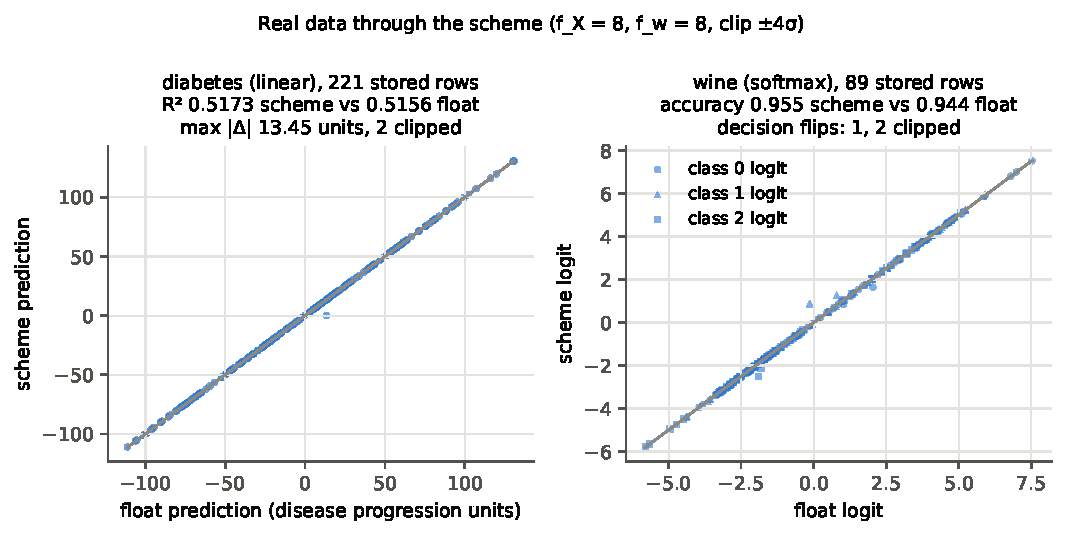
\includegraphics[width=\columnwidth]{fig1_real_scatter}
\caption{Real data through the scheme: each point is one stored row (one per class logit
for wine).}
\label{fig:real}
\end{figure}

\begin{table*}[t]
\centering
\caption{Real data at selected formats.}
\label{tab:real}
\begin{tabular}{llrrrrrrl}
\toprule
data & $f_X/f_w$, clip & $\log_2 q$ & $h$ & $m$ & clipped & max err & flips & metric (float $\to$ scheme) \\
\midrule
diabetes & 4/4, $\pm4\sigma$ & 14.3 & 0.288 & 1{,}579 & 2 & 0.166 & -- & $R^2$ 0.5156 $\to$ 0.5161 \\
diabetes & 6/6, $\pm4\sigma$ & 18.3 & 0.282 & 1{,}592 & 2 & 0.128 & -- & $R^2$ 0.5156 $\to$ 0.5169 \\
diabetes & 8/8, $\pm4\sigma$ & 22.3 & 0.254 & 1{,}656 & 2 & 0.182 & -- & $R^2$ 0.5156 $\to$ 0.5173 \\
diabetes & 8/8, $\pm8\sigma$ & 23.3 & 0.243 & 1{,}680 & 0 & 0.007 & -- & $R^2$ 0.5156 $\to$ 0.5158 \\
\midrule
wine & 4/4, $\pm4\sigma$ & 14.7 & 0.326 & 786 & 2 & 1.053 & 1 & acc. 0.9438 $\to$ 0.9551 \\
wine & 6/6, $\pm4\sigma$ & 18.7 & 0.331 & 780 & 2 & 0.982 & 1 & acc. 0.9438 $\to$ 0.9551 \\
wine & 8/8, $\pm4\sigma$ & 22.7 & 0.292 & 825 & 2 & 1.007 & 1 & acc. 0.9438 $\to$ 0.9551 \\
wine & 8/8, $\pm8\sigma$ & 23.7 & 0.280 & 839 & 0 & 0.020 & 0 & acc. 0.9438 $\to$ 0.9438 \\
\bottomrule
\end{tabular}

\end{table*}

\begin{figure*}[t]
\centering
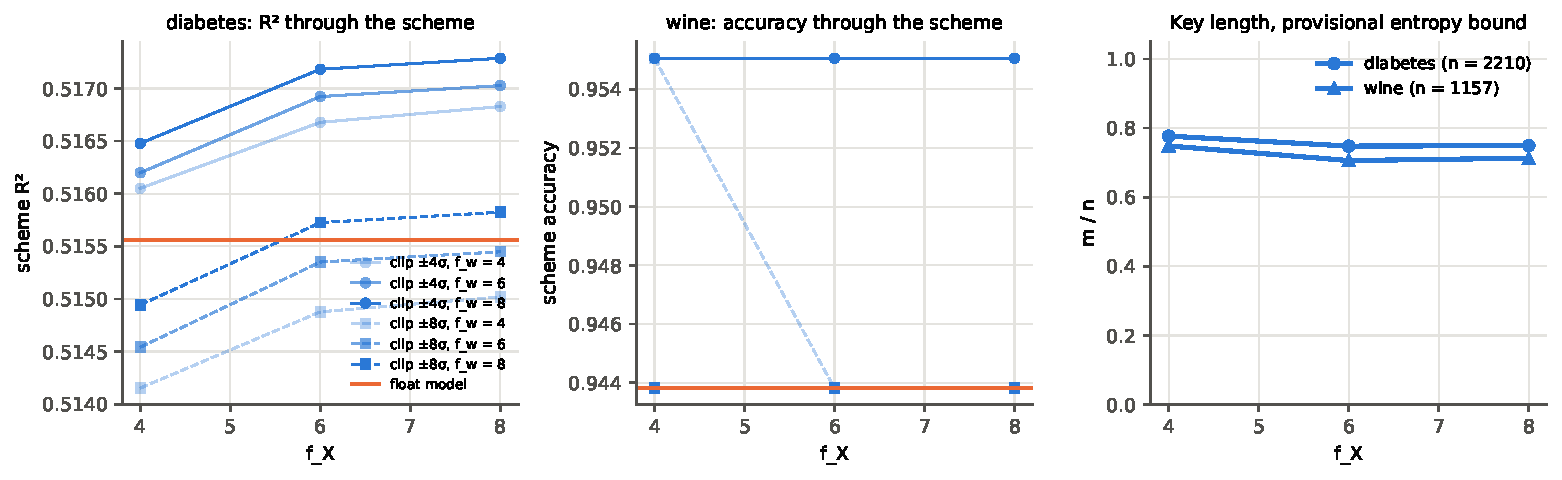
\includegraphics[width=\textwidth]{fig7_real_format}
\caption{Real data across formats: task metric (left, centre) and key length (right).}
\label{fig:realformat}
\end{figure*}

% ─────────────────────────────────────────────────────────────────────────────
\section{Limitations and future work}

\textbf{Adaptive queries.} Training by gradient descent sends queries that depend on
earlier results, which Observation~\ref{obs:inference} does not cover. Two directions are
open: queries built from data moments, and padding the weights with a fresh one-time pad
per request; the latter requires revisiting the ICC analysis.

\textbf{Real-data entropy.} The real-data key lengths rest on a Gaussian model of the
feature density. A model-free lower bound on $H_p(X)$ for correlated data would make them
unconditional.

\textbf{Scale.} One upload of $n$ values needs $\lambda=m+1\approx n(1-h)$ workers.
Splitting the data into independently keyed blocks would cap this, but needs a leakage
composition argument we leave to future work. Strongly correlated datasets such as breast
cancer (30 features, correlations up to $0.998$) are deferred for the same reason: their
min-entropy bound is far below the product of the marginals.

% ─────────────────────────────────────────────────────────────────────────────
\section{Conclusion}

Inference with a public model on stored data fits ICC without modification: the scores are
degree-one queries, the provider's view is the storage view, and fixed-point encoding gives
exact integers with an error the client chooses before upload. Across synthetic sources,
formats and two real datasets, the scheme's predictions matched the floating-point model
within the analytic bound, with a number of workers linear in the data size.

\bibliographystyle{IEEEtran}
\bibliography{refs}

\end{document}
